%!TEX root = main.tex

\section*{Introduction}

Genetic markers have long been used in the
management of Pacific salmon, and salmon conservation and management have been
at the forefront of a number of advances in molecular ecology,
from data generation techniques \citep{clemento2011discovery,campbell2015genotyping,mckinney2017managing,baetscher2018microhaplotypes}
to statistical methodology
\citep{smouse1990genetic,anderson2002model,pella2006gibbs,anderson2010assessing}.
Two broadly applicable techniques that have been
actively fostered by the Pacific salmon research community are genetic
stock identification
\citep[GSI:~][]{milner1982genetic,beacham2004dna,seeb2007development}
and parentage based tagging
\citep[PBT:~][]{anderson2006power, garza2007large, abadia2013large, steele2013validation}.



 In the 1980s, electrophoretically
detectable genetic variation, in the form of allozymes
\citep{ayala1972allozymes,allendorf1981use}, was used to
establish a program of GSI for Chinook salmon,
{\em Oncorhynchus tshawytscha} \citep{milner1982genetic}.  Extensive sampling
revealed that these allozyme markers
exhibited different allele frequencies among major lineages, or stocks, of Chinook salmon on the West Coast of the USA.
These allele frequency differences make GSI possible, and
\citet{milner1985genetic} soon showed that proportions of stocks in
the Washington state coastal troll fishery could be estimated by GSI\@.
Since that time, with the development of novel molecular markers, and, now
with increasing capacity to sequence genomic material, the scope and scale of GSI
has expanded considerably.

A critical ingredient for GSI is the {\em reference data set}, which consists of individuals
sampled from across a range of populations and with each individual genotyped using the same
panel of genetic markers.  When individuals of unknown origin are genotyped
at the same panel of genetic markers, the availability of the reference data set
makes it possible to do inference regarding the population of origin of the
unknown individuals.  Such reference data sets have seen widespread use and
development in salmon management, where they are often called
``genetic baselines," and defined as, ``databases of genotypes from
breeding populations"\citep{seeb2007development}.  Throughout, we will
use ``reference" or ``reference data set'' and ``baseline'' interchangeably; however,
a key point to keep in mind is that as genetic technologies
evolve over time, reference data sets continue to be developed and
refined to exploit the new technologies.  


By using greater numbers of more variable markers than the allozymes available
in the 1980s it is possible to accurately
identify the population of origin of individual fish, rather than simply estimating
aggregated stock proportions.  It is also possible to resolve populations of fish that
are much more closely related than before.  Furthermore, reference data sets with genotypes
from hundreds of populations throughout the range of multiple species of salmon and
other anadromous species
\citep{seeb2007development,gilbey2018microsatellite,barclay2019genetic} now exist, and are routinely used to assign fish caught thousands of
kilometers from their natal streams to their stock of origin. Applications include estimating fishery
composition \citep{satterthwaite2015stock}, providing real-time information for genetics-informed fishery closures \citep{beacham2004dna}, assessing the spatial distribution of different stocks in the
ocean \citep{urawa2009stock} and their temporal distribution in upstream migrations
\citep{hess2014monitoring},  and monitoring  bycatch \citep{hasselman2016genetic} or illegal captures \citep{wilmot1999origins} in marine fisheries.

Although sequencing costs continue to decline, they are high enough
that there remains a tradeoff
between reference baselines that include information from a large number of
populations across a broad scale, and those that have been tailored
to distinguish between closely related populations on a smaller, regional scale.
Because of cost considerations, reference baselines that include populations across a broad
spatial scale may include only a few populations from each sub-region.  Furthermore,
baselines tailored to a specific region often assemble markers that
show allele frequency differences between the closely related---and hence difficult
to resolve---stocks within the region.  Consequently, regionally targeted baselines typically
outperform broad-scale baselines in resolving populations within the region.

Over the last decade an additional genetic method, parentage based tagging, or PBT,
\citep{anderson2005description,steele2019parentage}
has become established as an extremely valuable management
tool for Pacific salmon.  The availability of such family-based methods adds another factor to
consider when developing a GSI baseline.
Since the first proposal \citep{anderson2005description} to replace or augment the coded-wire tag
programme \citep{nandor2010overview}
with PBT, it has been noted that one of the major advantages of a genetic program for
PBT is that the genetic markers used for PBT could also be useful for GSI (and
vice versa).
Thus, any panel of markers to be used for GSI (or PBT) should also be evaluated on its
utility for PBT (or GSI).

PBT has been remarkably successful in fisheries
management, having been used for over a decade in the management of Chinook salmon
and steelhead trout in major basins of the Columbia River \citep{steele2019parentage,horn2023multigeneration}, and having been employed to dramatically further our
understanding of the genetic inheritance of key traits in salmonids
\citep{abadia2013large,beulke2023distinct}. However, PBT is just one subset of a whole
family of statistical genetic methods employing relationship inference to learn about
populations.  For example, inference of the full siblings amongst a sample of fish
provides information about the effective number of adults producing offspring
\citep{waples2011inbreeding,wang2023estimating}, which can
be a valuable source of information when sampling of the adults is not possible.
Accordingly, marker panels should also be evaluated on their
capacity to resolve full-sibling relationships.

Chinook salmon are the largest of the Pacific salmonids and have historically been the target of extremely high-value and culturally important
fisheries \citep{myers1998status}. Moreover, because of their high degree of ecotypic variation, they have provided fishery opportunities in many
different seasons and geographic locations \citep{healey1991life}. However, recent declines in population sizes, from the Yukon River in the Arctic north,
to the southern extent of their range in California, has led to multiple fishery closures to protect
less productive stocks \citep{lindley2009caused}. The co-occurence of fish from relatively productive and relict populations reaches its paragon in California,
with the largest remaining ocean fisheries for Chinook salmon targeting the Central Valley fall-run stock that spawns in different tributaries of the
same river basin as the highly endangered and phenotypically distinct winter-run stock and the threatened spring-run stocks \citep{satterthwaite2015stock}.

Here, we present a reference baseline for Chinook salmon, focusing on the regional scale of
rivers within the state of California, and particularly targeted to the complex population
structure of Chinook salmon within the California Central Valley (CCV). Chinook salmon of the two main CCV river basins---the
Sacramento and the San Joaquin---exhibit the greatest run-timing diversity
within the species.  With four recognized ecotypes, delineated primarily on the basis of run timing
(fall-, late-fall-, winter-, and spring-run), adult Chinook salmon can be found migrating or residing
in freshwater every month of the year in California \citep{fisher1994past}.  


In spite of their distinct phenotypes and life history patterns, the four ecotypes of Chinook salmon in the Central Valley are closely related
\citep{clemento2014evaluation} and share recent common ancestry that is independent of ongoing migration between these lineages. As such, GSI
has been particularly challenging in the CCV, with at least one of the distinct ecotypes, the late-fall-run, unresolvable with previous GSI marker sets
and with unsatisfactory power for discriminating the protected spring-run stocks from the
harvested fall-run stock \citep{seeb2007development,clemento2014evaluation}.

We present a new reference baseline that includes 1,636 Chinook salmon individuals from 17 collections that were genotyped at 204 loci distributed throughout the genome.
This baseline is highly effective for GSI within California and provides ample power for PBT, thus enabling a highly effective and efficient integrated GSI/PBT monitoring and evaluation program 
\citep{garza2007large,beacham2021parentage}.
We describe how we identified and compiled the markers, including several new markers
identified through re-analysis of the whole genome sequencing data of \citet{thompson2020complex},
that are particularly effective at distinguishing between closely related groups of fish,
such as late-fall and fall-run Chinook salmon in the CCV.  We also provide a comprehensive analysis of this
set of markers for inference of parents and siblings within different groups of populations.



 \section*{Methods}

\subsection*{Population Sampling}

Samples of fish for the reference baseline were compiled from 13 locations within California, and one
within Oregon. This set of populations and stocks includes all of the previously described lineages of Chinook salmon in the southern portion of the range and most of the populations that are known to have significant genetic differentiation in this region.
These locations included sites in the two
main tributaries (the Sacramento River and the San Joaquin River) within
California's Central Valley, and the two main tributaries (Klamath and Trinity Rivers) in the Klamath basin in Northern California, and
three rivers of the California coast (Russian, Eel, and Smith).
Of the 1594 total fish samples from 17 different populations, 724 fish from 10 collections were of the fall run ecotype,
498 fish from 5 collections were spring run, and 261 and 111 fish were of the winter run and late-fall run ecotypes, 
respectively,  each represented by a single collection.
(Figure~\ref{fig:map}, Table~\ref{tab:samples}).
%%%%%%%%%%%%%
\begin{figure}
\newcommand{\mapcap}{\footnotesize  A map of sampling locations represented in the reference
baseline.  The colored circles aside
each location name represent the different run-timing groups of Chinook salmon
included in the collections from the location.  Color codes are as follows: \Wball~=~Winter run,
\LFball{}~=~Late-fall run, \Fball~=~Fall run, \Sball~=~Spring run.
Names of each location are followed by the location codes (Table~\ref{tab:samples}).
Abbreviations used in location names as follows:
R. = River; Ck. = Creek; H. = Hatchery; NFH = National Fish Hatchery.}
\begin{center}
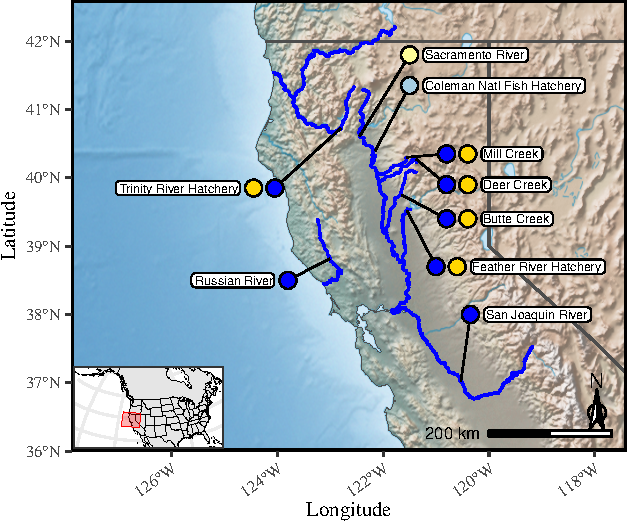
\includegraphics[width=0.48\textwidth]{images/map-crop.pdf}
\end{center}
\caption[\mapcap]{\mapcap}
\label{fig:map}
\end{figure}
%%%%%%%%%%%%%%%

Collections in each location were separated into fish from the different adult migration timing ecotypes according
to a variety of criteria.  Winter-run Chinook salmon are propagated at the Livingston
Stone National Fish Hatchery for supplementation (released as juveniles into the river) and as a captive broodstock;
sampling of this population was performed by hatchery staff during spawning. In Central Valley rivers with both
spring-run and fall-run ecotypes (i.e. Mill, Deer and Butte Creeks), previous research has documented different  (but overlapping) ranges of spawning time (Julian date) for each ecotype \citep{fry1961king,yoshiyama1998historical}.
As such, sampling targeted carcasses found in each of these
rivers at times representative of their run-timing designation, which were further confirmed using their genotypes
within the region of strongest association (RoSA) on chromosome 28 \citep{thompson2020complex}.
In the San Joaquin River, in 2016, at the time of sampling, only
fall-run Chinook salmon adults were found, therefore the samples could be categorized.  Run-timing
designation at the Feather River Hatchery is more complicated but it is managed by the hatchery practices in place:
early returning fish in May and April (expressing the spring-run life history) are visibly tagged and returned
to the river. Subsequently in the fall, when hatchery raceways are reopened, only fish with the visible tag are included
as spring-run broodstock, and the rest are included in the fall-run broodstock.
Putative spring-run and fall-run fish 
from these two broodstocks were sampled. Similar to broodstock collections in the CCV, samples from spring- and fall-run fish in the Trinity River were selected on the basis of spawn timing at the Trinity River Hatchery with migration-timing ecotype confirmed by RoSA genotype. Elsewhere, adult samples were taken from live broodstock at Rowdy Creek (Smith River), Iron Gate (Klamath River) and Warm Springs (Russian River) Hatcheries and juveniles were sampled from Blue Creek (Klamath River); all locations where only fall-run fish have been documented.  Spring run adult fish were sampled from the spring-run broodstock at Cole Rivers Hatchery on the Rogue River. Samples from the Eel River were taken from live fish ascending a ladder in the upper basin and were confirmed as fall-run ecotype by RoSA genotype. 



In total, the samples in the baseline represent fish from five (Table~\ref{tab:samples}) different Evolutionarily Significant
Units (ESUs) of Chinook salmon \citep{waples1991pacific}.
%%%%%%%%%%%%%%%%
\begin{sidewaystable*}
\caption{\footnotesize Collections of fish in the reference baseline.  The Sampling Months column shows
a pictorial representation of the proportion of each collection sampled in each month. BCkF were sampled as juveniles, all other collections were of adults. Colors in
this column correspond to run-timing groups as described in the caption of Figure~\protect\ref{fig:map}.}
\label{tab:samples}
{\small
\begin{tabular*}{\linewidth}{@{\extracolsep{\fill}} lllllllrcr}
\hline\hline
\vspace*{0.4ex}
Mainstem River$^1$&Code&Location Name$^2$&Run&Reporting Unit$^4$&ESU$^4$&$N$&$N_\mathrm{day}^5$&Sampling Months&Year Range\tabularnewline
\hline Rogue R.&CRHS&Cole Rivers H.&Spring&SO-NCal-Coast&SONCC&50&0&\raisebox{-0.12 em}{
\includegraphics[height=1.02em]{../tex/images/months-CRHS_Cole-Rivers-Hatchery.pdf}}&2004--2010\tabularnewline
Smith R.&SmRF&Smith R.&Fall&SO-NCal-Coast&SONCC&46&46&\raisebox{-0.12 em}{
\includegraphics[height=1.02em]{../tex/images/months-SmRF_Smith-River.pdf}}&2010--2011\tabularnewline
Klamath R.&BCkF&Blue Ck.&Fall&SO-NCal-Coast&SONCC&56&56&\raisebox{-0.12 em}{
\includegraphics[height=1.02em]{../tex/images/months-BCkF_Blue-Creek.pdf}}&2008--2008\tabularnewline
Klamath R.&IGHF&Iron Gate H.&Fall&Klamath-Trinity&UKTR&93&92&\raisebox{-0.12 em}{
\includegraphics[height=1.02em]{../tex/images/months-IGHF_Iron-Gate-Hatchery.pdf}}&2017--2017\tabularnewline
Trinity R.&TRS&Trinity R. H.&Spring&Klamath-Trinity&UKTR&46&46&\raisebox{-0.12 em}{
\includegraphics[height=1.02em]{../tex/images/months-TRS_Trinity-River-Hatchery.pdf}}&2012--2012\tabularnewline
Trinity R.&TRF&Trinity R. H.&Fall&Klamath-Trinity&UKTR&41&41&\raisebox{-0.12 em}{
\includegraphics[height=1.02em]{../tex/images/months-TRF_Trinity-River-Hatchery.pdf}}&2012--2012\tabularnewline
Eel R.&ERF&Eel R.&Fall&Cent-Cal-Coast&CCC&93&0&\raisebox{-0.12 em}{
\includegraphics[height=1.02em]{../tex/images/months-ERF_Van-Arsdale-Fisheries-Station.pdf}}&2014--2014\tabularnewline
Russian R.&RRF&Warm Springs H.&Fall&Cent-Cal-Coast&CCC&92&92&\raisebox{-0.12 em}{
\includegraphics[height=1.02em]{../tex/images/months-RRF_Warm-Springs-Hatchery.pdf}}&2012--2012\tabularnewline
Sacramento R.&SRW&Livingston Stone NFH&Winter&CV-Winter&CVWR&111&20&\raisebox{-0.12 em}{
\includegraphics[height=1.02em]{../tex/images/months-SRW_Livingston-Stone-National-Fish-Hatchery.pdf}}&2013--2014\tabularnewline
Sacramento R.&BCS&Butte Ck.&Spring&CV-Spring&CVSR&116&116&\raisebox{-0.12 em}{
\includegraphics[height=1.02em]{../tex/images/months-BCS_Butte-Creek.pdf}}&2004--2017\tabularnewline
Sacramento R.&MDS&Deer Ck.&Spring&CV-Spring&CVSR&34&34&\raisebox{-0.12 em}{
\includegraphics[height=1.02em]{../tex/images/months-MDS_Deer-Creek.pdf}}&2002--2002\tabularnewline
Sacramento R.&MDS&Mill Ck.&Spring&CV-Spring&CVSR&50&50&\raisebox{-0.12 em}{
\includegraphics[height=1.02em]{../tex/images/months-MDS_Mill-Creek.pdf}}&2002--2004\tabularnewline
Sacramento R.&FRHS&Feather R. H.&Spring&CV-Fall&CVSR&202&202&\raisebox{-0.12 em}{
\includegraphics[height=1.02em]{../tex/images/months-FRHS_Feather-River-Hatchery.pdf}}&2010--2019\tabularnewline
Sacramento R.&FRHF&Feather R. H.&Fall&CV-Fall&CVFR&106&106&\raisebox{-0.12 em}{
\includegraphics[height=1.02em]{../tex/images/months-FRHF_Feather-River-Hatchery.pdf}}&2008--2010\tabularnewline
Sacramento R.&BCF&Butte Ck.&Fall&CV-Fall&CVFR&45&45&\raisebox{-0.12 em}{
\includegraphics[height=1.02em]{../tex/images/months-BCF_Butte-Creek.pdf}}&2004--2016\tabularnewline
Sacramento R.&MDF&Deer Ck.&Fall&CV-Fall&CVFR&24&24&\raisebox{-0.12 em}{
\includegraphics[height=1.02em]{../tex/images/months-MDF_Deer-Creek.pdf}}&2002--2004\tabularnewline
Sacramento R.&MDF&Mill Ck.&Fall&CV-Fall&CVFR&49&49&\raisebox{-0.12 em}{
\includegraphics[height=1.02em]{../tex/images/months-MDF_Mill-Creek.pdf}}&2002--2004\tabularnewline
San Joaquin R.&SJRF&San Joaquin R.&Fall&CV-Fall&CVFR&79&79&\raisebox{-0.12 em}{
\includegraphics[height=1.02em]{../tex/images/months-SJRF_San-Joaquin-River.pdf}}&2016--2016\tabularnewline
Sacramento R.&CHLF&Coleman NFH&Late-fall&CV-Late-Fall&CVFR&261&261&\raisebox{-0.12 em}{
\includegraphics[height=1.02em]{../tex/images/months-CHLF_Coleman-National-Fish-Hatchery.pdf}}&2011--2015\tabularnewline

\end{tabular*}
}
\rule{3cm}{0.3pt}

{\scriptsize
$^1$R. = River.\\
$^2$Ck. = Creek; NFH = National Fish Hatchery; R. = River; H. = Hatchery.\\
$^3$Reporting Unit = an aggregation of the collections into groups relevant to management and
which are accurately resoluble with the genetic data in the baseline.
$^4$ESU = Evolutionarily Significant Unit; CVFR = Central Valley Fall Run ESU; CVSR = Central Valley Spring Run ESU; CVWR =
Central Valley Winter Run ESU; CC = California Coastal ESU; UKTR = Upper Klamath and Trinity Rivers ESU. \\
$^5N_\mathrm{day}$: the number of samples for which the specific sampling day was recorded.
}
\hrule\vspace*{0.3ex}\hrule
\end{sidewaystable*}
%%%%%%%%%%%%%%%%%%%%%

\subsection*{Genetic Markers}

The genetic markers in the baseline include newly discovered microhaplotypes, SNP assays
that were translated into amplicons, markers associated with phenotypes, and
species- and sex-specific markers.
These genetic markers were compiled from several different
efforts, as detailed in the sections below.

\subsubsection*{Novel microhaplotype discovery}

Candidate loci with multiple single-nucleotide polymorphisms (SNPs) among multiple
populations were identified using reduced-representation genome sequencing of 2--4 Chinook salmon, each, from a number of
populations ranging from California to British
Columbia and the interior Columbia River (Table~\ref{tab:ascert-panel}).
Genomic DNA was extracted using Qiagen DNeasy 96 Blood and Tissue Kits on a BioRobot 3000
(Qiagen, Inc). Double-digest restriction-site associated DNA sequencing (ddRAD) with different size selections (400 bp and 500 bp
fragments) were used to produce a broad array of locus targets. Library preparation and sequencing methods followed those of
\citet{peterson2012double} with the modifications described in \citep{baetscher2018microhaplotypes}.
Sequencing was performed on a MiSeq (Illumina, Inc) using $2 \times 300$-cycle paired-end sequencing.

Stacks v1.45 \citep{catchen2013stacks} was used to analyze the ddRAD sequence data.  As there was not a well-assembled Chinook salmon genome
at the time, the ustacks module of Stacks were used to assemble reads {\em de novo} into RAD loci.  Initial filtering retained RAD loci with two or more SNPs present
in at least 10 samples. After this initial filtering, there were 3,931 RAD loci retained in the ddRAD data with 400 bp size selection and
4,794 retained in the data with 500 bp size selection.
Gene regions were selected that (1) contained multiple SNPs within a 100 bp window, and (2) showed haplotype variation amongst the winter run and at least one other population.
A 100 bp window was used because the success of multiplex PCR and MiSeq sequencing is diminished in amplicons larger than 100 bp. Primer3
software \citep{untergasser2012primer3} was used to design primers for 229 gene regions that met these criteria.

These gene regions were PCR-amplified and sequenced on a MiSeq sequencer using a $2\times 75$-cycle kit.
The sequences from each locus were mapped to the {\em de novo} reference sequences (produced by Stacks) with
the Burrows-Wheeler aligner using the mem algorithm \citep{bwa-mem2009}. 
Subsequently, alignmets were sorted with SAMtools \citep{li2009sequence} and provided to
FreeBayes \citep{garrison2012haplotype} for variant calling.
FreeBayes output was filtered to remove indels and retain variants with a Phred-scaled quality score of 30
or greater and a read depth of 10 or higher. Further filtering and analysis of the loci, including
assessment of Hardy-Weinberg equilibrium \citep{hardy1908mendelian} was conducted in MICROHAPLOT (Ng {\em et al.}, DOI: 10.5281/zenodo.820110).  Loci that produced more than two haplotypes within an individual, and those clearly violating Hardy-Weinberg equilibrium within populations were removed.


\subsubsection*{Conversion of existing SNPtype assays}

A number of SNP markers from an earlier discovery effort \citep{clemento2011discovery} had already
been validated as useful for GSI
and PBT in California \citep{clemento2014evaluation}. These markers were originally assayed
using TaqMan (Life Technologies Corp., Carlsbad, CA) probes or SNPtype assays (Standard BioTools Inc., South San Francisco, CA).
These markers were typed using amplicon sequencing, following the methods in
\citet{campbell2015genotyping} with the addition of the Illumina small RNA sequencing primer and
read 2 sequencing primer to the SNPtype Specific Target Amplification Primer and Locus
Specific Primers respectively.  Loci were removed that were frequently inconsistent with SNPtype assays,
had poor amplification, or had excessive amplification and were subsequently over-represented in the sequencing library.  FreeBayes \citep{garrison2012haplotype} was used to identify all SNPs (additional to the TaqMan-assay targets) along the fragment, which facilitated scoring fragment microhaplotypes when multiple SNPs were present along the read \citep{baetscher2018microhaplotypes}. The resulting genetic markers are hereafter referred to as `SNPlicons' to record their origin as TaqMan assays in a previous
baseline.


\subsubsection*{Identifying the Late-Fall Associated Region (LFAR) and designing markers therein}

Loci with large allele frequency differences between late-fall and fall-run Chinook salmon,
were identified with a simple case-control genome-wide association study (GWAS) using the low-coverage whole-genome sequencing
data of \citet{thompson2020complex}, mapped to the Otsh\_v1.0 Chinook salmon assembly
(GenBank accession GCA\_002872995.1).  We conducted
two separate association-study comparisons.
The first involved the 16 late-fall-run fish as cases with 16 fall-run fish from the Feather River Hatchery as controls.
The second involved the same 16 late-fall fish as cases, but used 16 fall-run fish from the San
Joaquin River as controls.  The association studies were performed for each chromosome with
ANGSD \citep{pmid21663684,korneliussen_angsd_2014}, using the following command: {\footnotesize\tt angsd -yBin \{ybin\}  -r \{chrom\}
-minMapQ 30 -minQ 20 -minInd 12 -doAsso 1 -GL 1 -doMajorMinor 1 -doMaf 1 -SNP\_pval 1e-6
-out \{prefix\}  -bam \{bamlist\}}, where {\tt \{ybin\} } is the path to a file indicating the cases and
controls,
{\tt \{chrom\} } indicates the chromosome name, {\tt \{prefix\} } is the prefix to use for output files, and
{\tt \{bamlist\} } is the path to the text file holding paths to the binary alignment map (BAM) files
of aligned sequence data, one for each individual, ordered as in {\tt \{ybin\}}.

The GWAS $p$-values were compared relative to the commonly used significance threshold for
GWAS of $5\times 10^{-8}$ \citep{chen2021revisiting}.  Only a single site exceeded that threshold in both comparisons and it occurred
atop a peak in association scores on chromosome 34 (see
Results). Candidates for follow-up genotyping were identified in the peak by including the 10
SNPs in that peak with the lowest association $p$-values, and supplementing those with additional SNPs that
showed:
\begin{itemize}
\item An estimated absolute allele frequency difference between late-fall and all 32 fall-run fish, $|d| >0.75$,  with an approximate lower confidence interval of $|d|$ greater than 0.5,  or
\item $|d| >0.5$ with a lower confidence interval $>$0.25 and
with either fall-run or late-fall run being nearly fixed for one of the alleles, or
\item An annotation from snpEff \citep{cingolani2012program} of ``High'' or ``Moderate,'' or
\item $|d|>0.48$ and a lower confidence interval of $>$0.25 and a
genomic  coordinate $> 2.2$~Mb.
\end{itemize}
The final condition was implemented in order to gather several SNPs with large allele frequency differences
that were adjacent to, but not directly within, the main peak of association, so as to possibly learn about
recombination in the region.  

We designed amplification primers for the candidates using
Primer3 \citep{koressaar2007enhancements,untergasser2012primer3} and tested amplification in a
subset of Chinook salmon
samples. The primer pairs that amplified sequence that reliably mapped back to the association-peak region were typed
in a separate collection of 1,638 Sacramento River Chinook salmon sampled from the fish trap below Keswick Dam, including 1,169 winter run, 281 spring
run, and 188 fall/late-fall run. We divided the fish identified
from the 125-locus genetic
stock identification data set of \citet{thompson2020complex}  as fall/late-fall into fall run and late-fall run according
to their sampling date at Keswick:  99 fish arriving before Dec 26 were classified as fall run and 89 fish arriving after Dec 26 were
classified as late-fall run.   The allele frequencies of the target SNPs at the remaining amplicons
were
estimated for each of these four groups: winter, spring, fall, and late-fall, and
amplicons showing large allele frequency differences between late-fall fish and all other runs were retained.


\subsubsection*{Winter-run associated polymorphisms (WRAPs)}

Using the whole genome sequencing data of \citet{thompson2020complex}, we also sought
genomic regions that might provide diagnostic markers for the Sacramento winter-run
Chinook salmon.  This ecotype is highly differentiated from all other Chinook salmon populations
throughout its genome, which complicates the process of finding diverged genome regions using
a simple association study, with only 16 samples, as done to identify the LFAR.  Consequently we pursued a bespoke
analysis to find regions expected to have large allele frequency differences between
the winter-run and all other ecotypes of Chinook salmon in California's Central Valley.   This analysis
screened for regions with large allele frequency differences across large blocks of the genome, and is
described in the supplemental text section \ref{sec:wrap-methods}.

\subsubsection*{Adult-migration-timing associated markers}

We include six amplicons that capture the eight  SNPs within the ``Region of Strongest Assocation'' (RoSA)
between spring-run and fall-run fish, near the ROCK1 and GREB1L genes,  on Chromosome 28 listed in Table~S3 of \citet{thompson2020complex}.
We add three more amplicons in the same RoSA region to the panel, as well as one more amplicon that
allows genotyping of snp670329, which was discovered and described by \citet{thompson2019anthropogenic}.
Including all these markers in the panel allows them to be routinely typed, creating
 a database for understanding the spatial and temporal
distribution of the alleles in this genomic region; however these markers are omitted from likelihood calculations for
GSI, since their distribution across populations in the Feather River has been clearly and evidently
influenced by hatchery practices (see Results), it is not necessary to include them for accurate assignment,
and because the 12 SNPs within these three amplicons are typically in profound linkage disequilibrium (LD)
making them inappropriate for use as separate markers in most software for population assignment or GSI, that
typically assumes markers are not in LD within the component populations of the baseline.




\subsubsection*{Additional phenotypically associated markers}

The baseline also includes three amplicons with genetic variation
in two genes, VGLL3 and SIX6,
found to be associated with phenotypes related to reproductive maturity in both
Atlantic \citep{barson2015sex} and Pacific \citep{waters2021heterogeneous} salmonids. They
provide additional variation for population genetic analyses and to
monitor populations for potential phenotypic patterns.

We include an assay from a novel locus that targets the sex-determining region ({\em sdY}) on the Y chromosome in Chinook salmon. We designed this assay to target the SNP described by \citet{bertho2022nonfunctional} that differentiates the functional {\em sdY} and a nonfunctional {\em sdY} pseudogene.  Examination of whole-genome sequence data in multiple populations of California Chinook salmon \citep{thompson2020complex} shows that this
marker characterizes genetic sex in diverse California salmon populations more accurately than previously published assays  \citep{von2015development}.
Finally, marker Ots\_coho001\_05\_32691399, which is fixed for alternate alleles in
coho salmon and Chinook salmon, is included to diagnose when samplers have unwittingly
collected coho salmon.

\subsection*{Localizing markers within the genome}

The novel microhaplotype markers and the SNPlicon targets were
developed prior to the advent of a well-assembled genome for Chinook salmon.
As a consequence, many of these markers had
been used previously without certainty about their location in the genome.
After designing and validating an amplicon-sequencing approach to type both of these
groups of markers we identified their locations within the genome by mapping the
consensus sequences (roughly 100--300 bp) around the markers
to both the Chinook salmon version 1 (Otsh\_v1.0, GenBank accession GCA\_002872995.1)
and version 2  (Otsh\_v2.0, GenBank accession GCA\_018296145.1) genome assemblies,
using both bwa mem \citep{bwa-mem2009} and the BLAST-like Alignment tool, BLAT \citep{kent2002blat}.
A similar mapping exercise was performed for the remaining markers to
report their locations in both Otsh\_v1.0 and Otsh\_v2.0.


\subsection*{Amplicon sequencing, microhaplotype calling, and further quality control}

Amplicon sequencing was performed with the Genotyping-in-Thousands-by-sequencing (GT-seq)
method \citep{campbell2015genotyping}. All loci were
multiplexed with primer concentrations ranging from 0.083 uM to 0.5 uM to increase
uniformity of read depths across all loci. Sample normalization was
performed using the SequalPrep Normalization Plate Kit (Applied Biosystems) according
to the manufacturer's instructions. Samples were pooled by plate
and purified using Agencourt AMPure XP magnetic beads.
Libraries were quantified either by qPCR with the NEBNext Library Quant Kit for Illumina (New
England BioLabs) or with the Qubit dsDNA HS Assay Kit (Thermo Fisher Scientific)
before dilution and pooling for sequencing.
All samples were sequenced on a MiSeq using $2\times 75$-cycle paired-end sequencing protocols.
Primer sequences and concentrations for making the primer pool are in Supplemental Data~1.

For evaluation of candidate loci, dual-barcoded sequences were used
to identify individual tissue samples using the MiSeq analysis software (Illumina).
The paired-end sequence reads were joined together using Fast Length Adjustment
of SHort reads \citep[FLASH:~][]{magovc2011flash} and mapped to an indexed sequence reference created from the Stacks target loci (for the novel microhaplotypes, SNPlicons and RoSA markers) or from the entire Otsh\_v1.0 genome
(for the LFAR, WRAP, VGLL3, and Six6 markers) using bwa mem. Mapped reads were converted to BAM files using SAMtools and FreeBayes was used to call variants.

For genotyping of baseline samples, final filtering at each locus required a read depth of 20 and a read depth ratio of 0.30 (i.e., for heterozygotes the lower read depth haplotype must have 30\% of the total reads at that locus). MICROHAPLOT was used to call alleles and genotype processing was performed with R scripts.

Each locus was assessed for the presence of null alleles using the R package `whoa'
\citep[\url{https://github.com/eriqande/whoa};  see][]{hendricks2018recent}.

\subsection*{Population genetic analyses}

Basic data summaries were calculated for each population/collection
in the reference baseline
using simple operations in the R programming language, Version 4.3
\citep{rcore}. Summaries provided are:
\begin {itemize}
\item the average over loci of the number of fish
in which each locus was successfully genotyped, $\bar{N}$;
\item the average number of alleles per locus in each collection with all collections
downsampled to the smallest number of genotyped individuals at each
locus, $\bar{N}_\mathrm{A,ss}$;
\item the fraction of polymorphic
loci in each collection after subsampling to the smallest number of genotyped
fish, $\bar{P}_\mathrm{poly,ss}$;
\item the expected heterozygosity as the average over loci
of one minus the frequencies of homozygotes at each locus expected from the
estimated allele frequencies, $\bar{H}_\mathrm{exp}$; and
\item the observed heterozygosity as the average over
loci of the fraction of heterozygous genotypes, $\bar{H}_\mathrm{obs}$.
\end{itemize}
When subsampling each collection to the minimum number of genotyped
fish across all collections at a locus, individuals were subsampled without
replacement, taking the average of 1,000 different random subsamples.

We calculated \citet{weir1984estimating}'s pairwise $F_\mathrm{ST}$ between
all collections, using the {\footnotesize\tt pp.fst} function from the R
package `hierfstat' \citep{hierfstat}. Population
structure in the data was evaluated
using the program STRUCTURE \citep{pritchard2000inference,falush2003inference}.
For this analysis, we omitted the run-timing associated markers.
We performed 20 replicate runs at each value of the assumed number of
subpopulations, $K$, in $\{2, 3, 4, 5, 6, 7\}$
using default settings of the program.  STRUCTURE output was
summarized and visualized using CLUMPAK
\citep{kopelman2015clumpak}.






\subsection*{Power for genetic stock identification and population assignment}

To assess the power of the marker panel for GSI, we used the R package
`rubias' \citep{moran2019bayesian}.  The function {\tt self\_assign()} was used
to assign each individual in the reference baseline to one of the
collections within the baseline.  Each fish was removed from the reference baseline
when calculating the likelihood that it originated from the collection it actually belongs
to, using a classical leave-one-out approach to eliminate the inflated estimates of
power that might occur without such a procedure \citep{anderson2008improved}.
The scaled likelihoods of collection membership returned by
{\tt self\_assign()} were summed within reporting units, and fish were
assigned to the reporting unit with the largest value of that sum.  Subsequently,
fish were assigned to the collection within that reporting unit with the highest
scaled likelihood.  We considered two thresholds for assignment.  In the first,
all fish are assigned, in the second only fish with a summed (i.e., summed
over all collections in a reporting unit)
scaled likelihood greater than 0.8 were assigned.

Finally, we investigated the matrix of assignments and misassignments
broken down according to the genotype of the fish at the markers within
the RoSA.  RoSA genotype \citep[EE, EL, or LL, see~][]{thompson2020complex}
was assessed from the concordance of the genotypes
at all 8 markers described in \citep{thompson2020complex}, requiring that no genotypes be missing
within an individual from any of those 8 markers, and discarding data from 12 individuals
in which the E or L haplotypes had clearly recombined.



\subsection*{Power for relationship inference}

To explore the utility of the marker panel for relationship inference, we used
the R package `CKMRsim'
(\url{https://github.com/eriqande/CKMRsim})
to estimate the false-positive rates (FPRs) expected at
different values of the false negative rate (FNR) for a variety of different pairwise
relationships in different populations.  For these purposes, collections were divided into
10 different groups.  The members of each group are
relatively, genetically similar, but the groups do not necessarily correspond to reporting
units, because, in some cases, FPRs and FNRs are desired for a single
collection.   The assumed genotyping error rate
was 1\% per locus and the genotyping error model was the default
"True-genotype-independent" model.


For errors of misidentifying
unrelated (U) pairs as parent-offspring (PO), full-sibling (FS), or half-sibling (HS)
pairs we used importance sampling to estimate the very small FPRs.  The
FNRs were estimated in each case using simple Monte Carlo taking account
of the physical linkage of the markers by inputting their genomic positions into
`CKMRsim' and using the package's interface to the MENDEL \citep{lange2013mendel}
software to simulate genotypes of related pairs
in the presence of physical linkage.  
For errors of misidentifications between the relationship
types of avuncular (AN: aunt-niece, uncle-nephew, etc.), PO, FS, and HS,
we used regular Monte Carlo to estimate the FPRs and FNRs, because
importance sampling cannot be used in those cases. Since there are
expected to be far fewer such relationships than the number of unrelated
pairs, the relevant FPRs are large enough that they can be reliably estimated
(at least down to rates of $10^{-3}$) without importance sampling.
For AN, FS, and HS, both the
FPRs and FNRs were estimated while taking account of physical linkage
of the markers, as described above.

\section*{Results}

\subsection*{Genetic Markers}

%%%%%%%%%%%%%%%%%%%%%%%%%%%%%%%%%%%
\begin{table}
\caption{\footnotesize  Summary of amplicons in the reference data set.  Source denotes
which discovery effort yielded the amplicon. N (amplicon) is the number of amplicons
and N (variant) is the total number of variant sites routinely assayed within the sequence of each
amplicon.  Source abbreviations are as follows: mhap = novel microhaplotype discovery, scon = conversion of existing SNPtype
assays, rosa = adult-migration-timing associated markers, wrap = winter-run associated
polymorphisms, lfar = late-fall-run associated polymorphisms, sixx and vgll = amplicons
targeting the SIX6 and VGLL3 genes, respectively, sexy = sexID marker, coho =
distinguishes coho from Chinook salmon. The $^*$ denotes markers routinely
excluded from likelihood calculations for GSI.}
\label{tab:loci-summ}
{
\begin{tabular*}{0.48\textwidth}{@{\extracolsep{\fill}} lrr}
\hline\hline
Type&N (amplicon)&N (variant)\tabularnewline
\hline
mhap&106&458\tabularnewline
scon&78&200\tabularnewline
rosa$^*$&10&22\tabularnewline
wrap&3&7\tabularnewline
lfar&2&6\tabularnewline
sixx&2&2\tabularnewline
coho$^*$&1&2\tabularnewline
sexy$^*$&1&\tabularnewline
vgll&1&1\tabularnewline
\end{tabular*}
}
\vspace*{-2.3ex}\hrule width0.48\textwidth
\vspace*{0.3ex}\hrule width0.48\textwidth
\end{table}
%%%%%%%%%%%%%%%

A summary, which includes genomic location, consensus sequence, and primer sequences,
of all the amplicons used in the baseline is available
in Data Supplement~1.  An overview of genomic coordinates is found in Figure~\ref{fig:genome-locations}

\subsubsection*{Additional microhaplotype discovery}

Of 229 tested candidates from our novel microhaplotype discovery process
125 markers were retained \citep{thompson2020complex}
for use in stock identification within
the Klamath Basin.  However, further evaluation of those markers in other
populations led the removal of
twelve loci with apparent null alleles in the winter-run population, two that were monomorphic
in the winter-run, despite having
multiple alleles in other populations, and an additional 5 loci that were
difficult to score in routine application of the baseline. This left 106
novel microhaplotype amplicons in the current panel.


\subsubsection*{Conversion of existing SNPtype assays}

Of the 96 existing SNPtype assays, we were able to convert 78
into reliable amplicon-sequenced assays that were included in the panel.



\subsubsection*{Late-fall Associated Region Markers}

The case-control association identified only a single SNP with $p < 5\times 10^{-8}$ in the comparison
between late-fall run and both the FRH fall-run and the San Joaquin fall run.  This SNP was within
a single evident peak on chromosome 34 with large allele frequency differences
between Central Valley late-fall and fall-run fish.  This peak was evident both in the comparison of
late-fall fish to fall-run fish in the Feather River Hatchery and of late-fall fish to the fall-run fish in
the San Joaquin River (Figure~\ref{fig:lfar-assoc}).




The Manhattan plot of Figure~\ref{fig:lfar-assoc} shows sporadic SNPs with low association
$p$-values.  These are not shared between the two different late-fall to fall comparisons, and
were concentrated in areas of poor mapping, suggesting that their
$p$-values were artifactual.  By contrast, a large number of sites near the prominent peak on
chromosome 34 had large allele frequency differences between late-fall and fall run.  Taking the
10 SNPs with the lowest association $p$-values, and including additional ones from the filtering criteria given in the
Methods, yielded 49 candidate markers for which we designed primers for amplification (Figure~\ref{fig:lfar-candi}).  Only 8
of these 49 primer pairs yielded reliable amplification and mapping.   Of these 8, two of the SNPs
showed inconsistent genotyping and were removed from consideration.  Of the remaining 6, only 3
showed marked allele frequency differences ($> 0.7$) between late-fall and fall run.  These three
SNPs (located at: Chr34:828,768,  Chr34:865,057, and Chr34:1,063,084 in the Otsh\_v1.0 assembly)
also had pronounced differences in allele frequency between
late-fall and spring or winter run.

Analysis of the mapping of amplicons for Chr34:828,768
showed that many ($\approx$89\%) of the reads were off-target (aligning to other chromosomes,
etc.), making it costly (in terms of sequencing effort) to include the marker in the baseline panel.
Consequently it was dropped from the panel.  The two remaining loci, which are at coordinates
Chr34:865,057, and Chr34:1,063,084 in the Otsh\_v1.0 assembly are at coordinates
Chr34:954,054 and  Chr34:1,151,868 in the Otsh\_v2.0 assembly, and
the frequency of the different alleles at the two remaining loci
within different reporting units in the baseline are shown in Table~\ref{tab:lfar-freqs}.
%%%%%%%%%%%%%%
\begin{table}
\caption{\footnotesize Allele frequencies across reporting units of the two late-fall associated
markers.  Frequencies are given for the alleles most common amongst late-fall Chinook: nucleotide
{\tt G} at locus Chr34:954,054 and {\tt A} at Chr34:1,151,868.  $N$ is the total number of gene
copies available for estimating the allele frequency. Genome coordinates of SNPs are from Otsh\_v2.0.}
\label{tab:lfar-freqs}
{\footnotesize
\begin{tabular*}{0.48\textwidth}{@{\extracolsep{\fill}} lrrrr}
\hline\hline
& \multicolumn{2}{c}{\underline{Chr34:954,054}} & \multicolumn{2}{c}{\underline{Chr34:1,151,868}} \\
Reporting Unit & freq. & $N$ & freq. & $N$ \\ \hline
CV-Late-Fall&0.750&516&0.733&592\tabularnewline
CV-Fall&0.054&910&0.030&908\tabularnewline
CV-Spring&0.023&396&0.003&396\tabularnewline
CV-Winter&0.005&222&0.005&222\tabularnewline
Cent. Cal. Coast&0.000&92&0.004&278\tabularnewline
Klamath-Trinity&0.000&172&0.000&358\tabularnewline
SO-Ncal-Coast&0.000&192&0.000&304\tabularnewline

\end{tabular*}
}
\vspace*{-2.3ex}\hrule width0.48\textwidth
\vspace*{0.3ex}\hrule width0.48\textwidth
\end{table}
%%%%%%%%%%%%%%%

\subsubsection*{Winter-run-associated polymorphisms}

Initial examination of sequence data 
in the 16 winter-run fish and 84 non-winter run fish revealed
a number of SNPs that were potentially diagnostic, but none were fixed for alternate alleles 
in a larger sample.
Nonetheless, three of these markers had large frequency differences
between the groups and are included in the reference baseline.  The process of 
discovering them is described in the supplemental text section \ref{sec:wrap-methods}.

\subsection*{Localizing markers within the genome}

Of the 184 loci that originated from our novel
microhaplotype discovery or from SNPtype assays, 179 of them were mapped by both bwa mem and
BLAT to exactly the same location
on an assembled chromosome in the Otsh\_v2.0 genome.
Of the remaining 5 loci, one of them was mapped to the same location by BLAT and bwa mem, but
the alignments differed in length, two of them had a single secondary alignment on a different chromosome
that was identical in both bwa mem and BLAT, one of them had only a fragment mapping to
the secondary alignment, and one of them had multiple
non-primary alignments (Supp.~Data~1).

Mapping to Otsh\_v1.0 was similar, except that a greater number of markers mapped to unplaced
scaffolds in Otsh\_v1.0 than in Otsh\_v2.0, likely reflecting the more complete nature of the
second assembly.


\subsection*{Population genetic summaries}

The total number of alleles per locus varied between 1 and 10 (Figure~\ref{fig:num-alle}), with the
only locus bearing a single allele in Chinook salmon being the species-specific marker Ots\_coho001\_05\_32691399. 
Biallelic loci were most common, at 66 of the total, but two-thirds of the microhaplotype markers
showed more than two alleles, which has been shown to provide significantly more
power for relationship inference than a comparably sized panel of biallelic SNPs
\citep{baetscher2018microhaplotypes}.


The population-genetic summary statistics are presented in Table~\ref{tab:pg-summ}.
%%%%%%%%%%%%%%
\begin{table}
\caption{\footnotesize Simple population genetic summaries. All quantities are means
over loci.  $\bar{N}$ is the average over loci of the number of fish in each collection with observed genotypes
at a locus; $\bar{N}_\mathrm{A,ss}$ is the
average number of alleles and $\bar{P}_\mathrm{poly,ss}$ the fraction of polymorphic loci,
after sub-sampling to the smallest sample size per locus; $\bar{H}_\mathrm{exp}$ and
$\bar{H}_\mathrm{obs}$ are expected and observed heterozygosity, respectively. Population
codes are as given in Table~\ref{tab:samples}}
\label{tab:pg-summ}
{\footnotesize
\begin{tabular*}{0.48\textwidth}{@{\extracolsep{\fill}} lrrrrr}
\hline\hline
Code&$M$&$\bar{N}_\mathrm{A,ss}$&$\bar{P}_\mathrm{poly,ss}$&$\bar{\mathrm{H}}_\mathrm{exp}$&$\bar{\mathrm{H}}_\mathrm{obs}$\tabularnewline
\hline CRHS&0.008&2.60&0.95&0.398&0.399\tabularnewline
SmRF&0.021&2.60&0.95&0.401&0.394\tabularnewline
BCkF&0.041&2.59&0.96&0.393&0.382\tabularnewline
IGHF&0.028&2.37&0.93&0.356&0.363\tabularnewline
TRS&0.036&2.37&0.92&0.353&0.348\tabularnewline
TRF&0.031&2.37&0.92&0.352&0.351\tabularnewline
ERF&0.022&2.51&0.95&0.364&0.356\tabularnewline
RRF&0.037&2.64&0.96&0.398&0.391\tabularnewline
SRW&0.338&2.32&0.88&0.338&0.329\tabularnewline
BCS&0.046&2.52&0.92&0.379&0.373\tabularnewline
MDS&0.082&2.55&0.94&0.394&0.397\tabularnewline
FRHS&0.108&2.61&0.95&0.397&0.392\tabularnewline
FRHF&0.029&2.63&0.96&0.394&0.398\tabularnewline
BCF&0.123&2.60&0.94&0.385&0.370\tabularnewline
MDF&0.130&2.59&0.94&0.386&0.383\tabularnewline
SJRF&0.012&2.57&0.94&0.384&0.380\tabularnewline
CHLF&0.068&2.53&0.94&0.386&0.384\tabularnewline

\end{tabular*}
}
\vspace*{-2.3ex}\hrule width0.48\textwidth
\vspace*{0.3ex}\hrule width0.48\textwidth
\end{table}
%%%%%%%%%%%%%%%
The average number of fish with non-missing data in each population varied from
a low of 40.2 (TRF) to a high of 279.6 (CHLF).  The average number of alleles
per locus, standardized to the smallest sample size, ranged from 2.32 (SRW) to
2.64 (RRF), with  SRW also having the smallest value of the
standardized fraction of polymorphic markers at 0.88 and RRF sharing the highest value
(0.96) with FHRF and BCkF.
SRW also had the lowest values for expected and observed heterozygosity:
0.338 and 0.329, respectively. While the highest for expected heterozygosity
was 0.401 (SmRF) and for observed heterozygosity, 0.399 (CRHS).

The estimated pairwise $F_\mathrm{ST}$ values between the collections
varied from a low of 0.0 to a high of 0.288 (Figure~\ref{fig:gsi}a).
Notably, most of the largest values
of $F_\mathrm{ST}$ occurred between SRW and another collection.
%%%%%%%%%%%%%%%%%%%%%%
\begin{figure}
\newcommand{\gsicap}{\footnotesize ({\bf a)} Pairwise $F_\mathrm{ST}$ values and allele frequencies,  
and ({\bf b)} self-assignment rates.  The codes of the populations
appear on the outer margins of the table atop cells colored according to the run-timing group
of the collection.  Interior cells are colored according to reporting unit.  In ({\bf a}), for $F_\mathrm{ST}$ values,
the upper triangle was computed using all the genetic markers except for those in the
RoSA on chromosome 28. 
Each cell in the lower triangle shows a small scatter plot of estimated allele frequencies
in the collections---the $x$ value is allele frequencies from the collection in the column and the
$y$ value is from the collection in the row. Frequencies for all alleles are shown, with values within
each cell ranging from 0 to 1.  These frequencies were estimated by, for each locus, randomly
subsampling individuals from each collection to the minimum number of observed alleles in any collection
at the locus.  In ({\bf b}), for self-assignment tallies, the row corresponds
to the true source collection and the column corresponds to the assigned collection.
All individuals were assigned here, using a maximum-scaled-likelihood rule to reporting unit and
to collection within reporting unit as described in the text. For the assignment matrix resulting
when only fish with a scaled likelihood $>0.80$ to reporting unit are assigned, see Figure~\ref{fig:eighty}}
\begin{center}
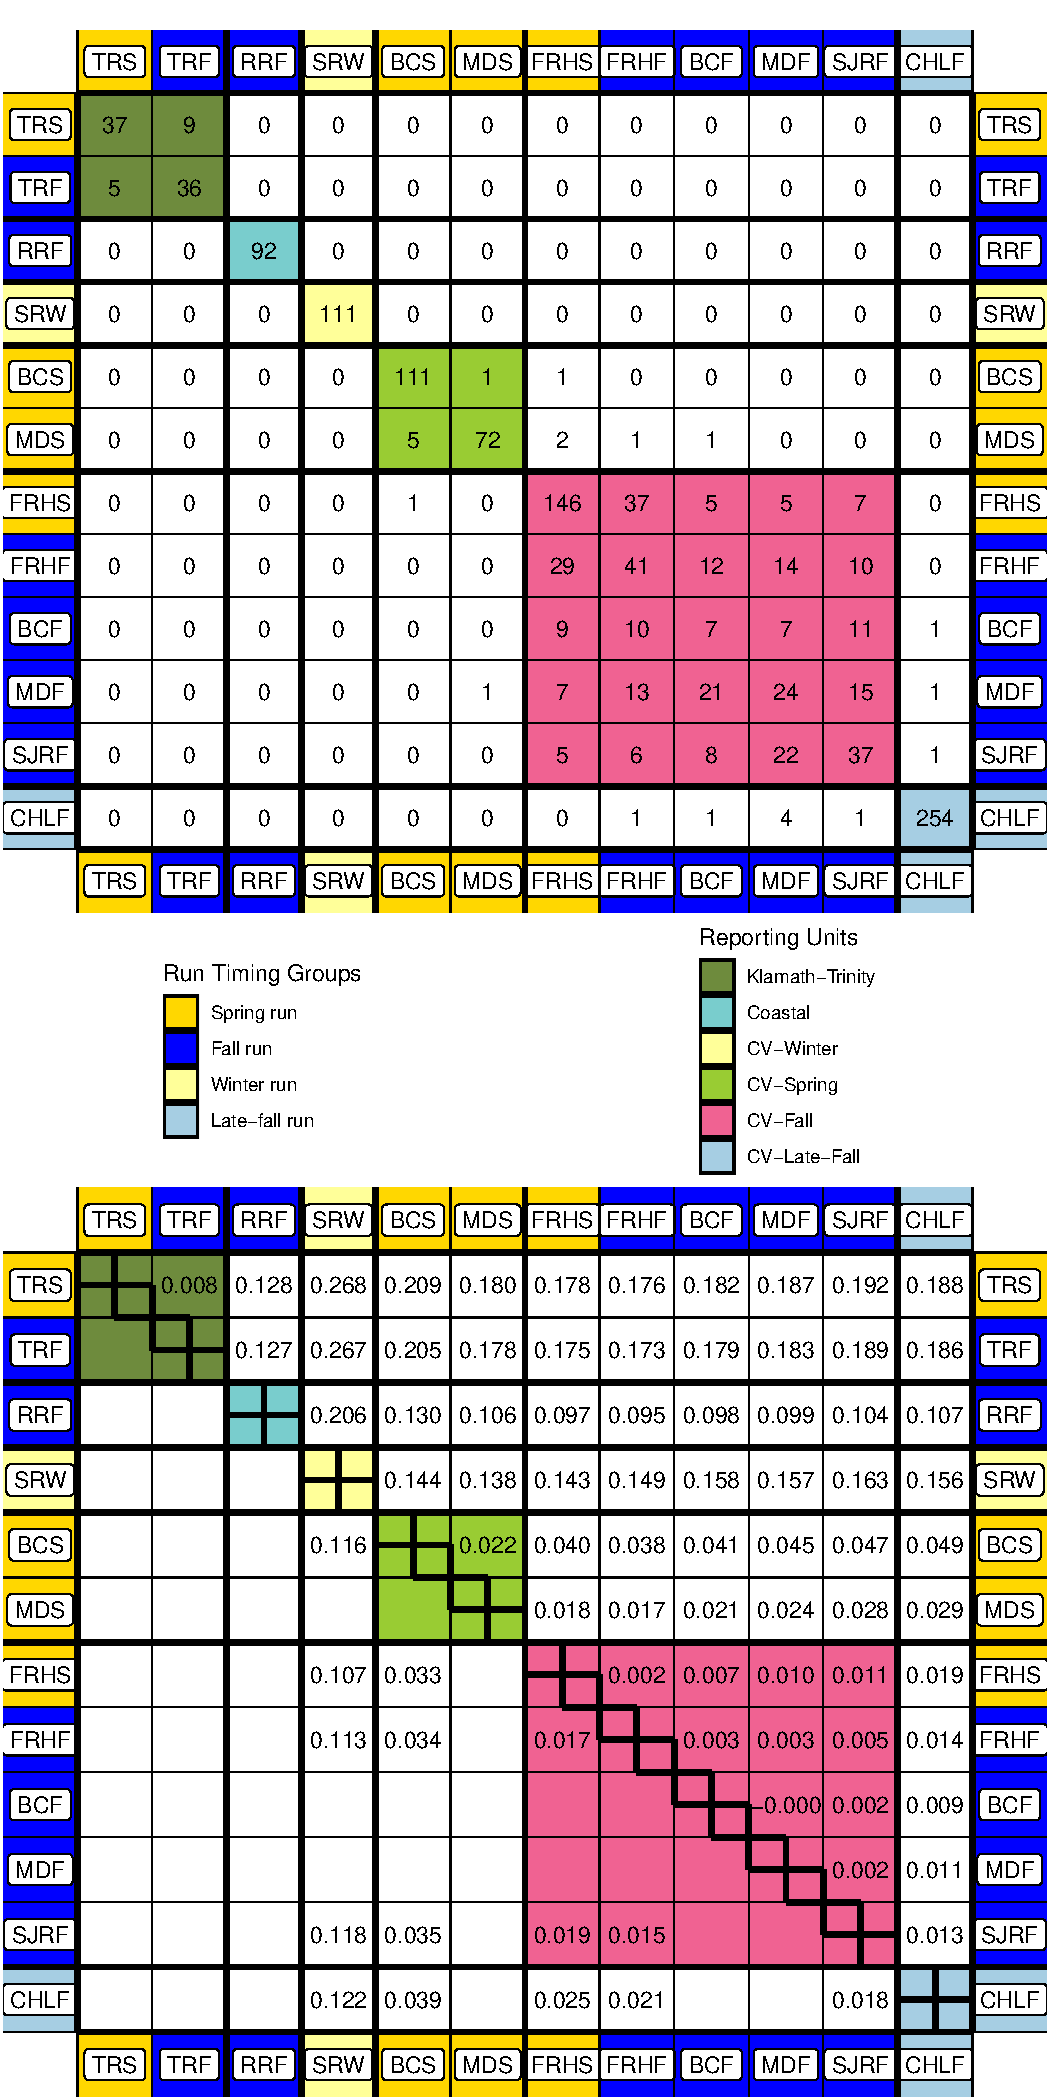
\includegraphics[width=0.48\textwidth]{images/gsi_and_fst_fig-crop.pdf}
\end{center}
\caption[\gsicap]{\gsicap}
\label{fig:gsi}
\end{figure}
%%%%%%%%%%%%%%%%%%%%



At values of $K$ from 2 to 7, clusters identified by the program STRUCTURE
generally corresponded to groupings of related populations, and confirmed
{\em a priori} knowledge about which collections in the baseline could and should be
grouped together into reporting units (Figure~\ref{fig:struct}).  At every value of $K$, CLUMPAK discerned at least
12 of 20 replicates in the major mode (Figure~\ref{fig:struct}).   
Clustering solutions in the minor
modes generally converged on a single alternative solution and appear in Figure~\ref{fig:minor-modes}.
%%%%%%%%%%%%%%%%%%%%
\begin{figure}
\newcommand{\structcap}{\footnotesize Major modes found by STRUCTURE and summarized
by CLUMPAK out of 20 replicates for each value of $K$, the assumed number of
subpopulations. $K$ value is listed at lower right of each barplot, followed by the number
of replicate runs of structure that converged to this major mode.}
\begin{center}
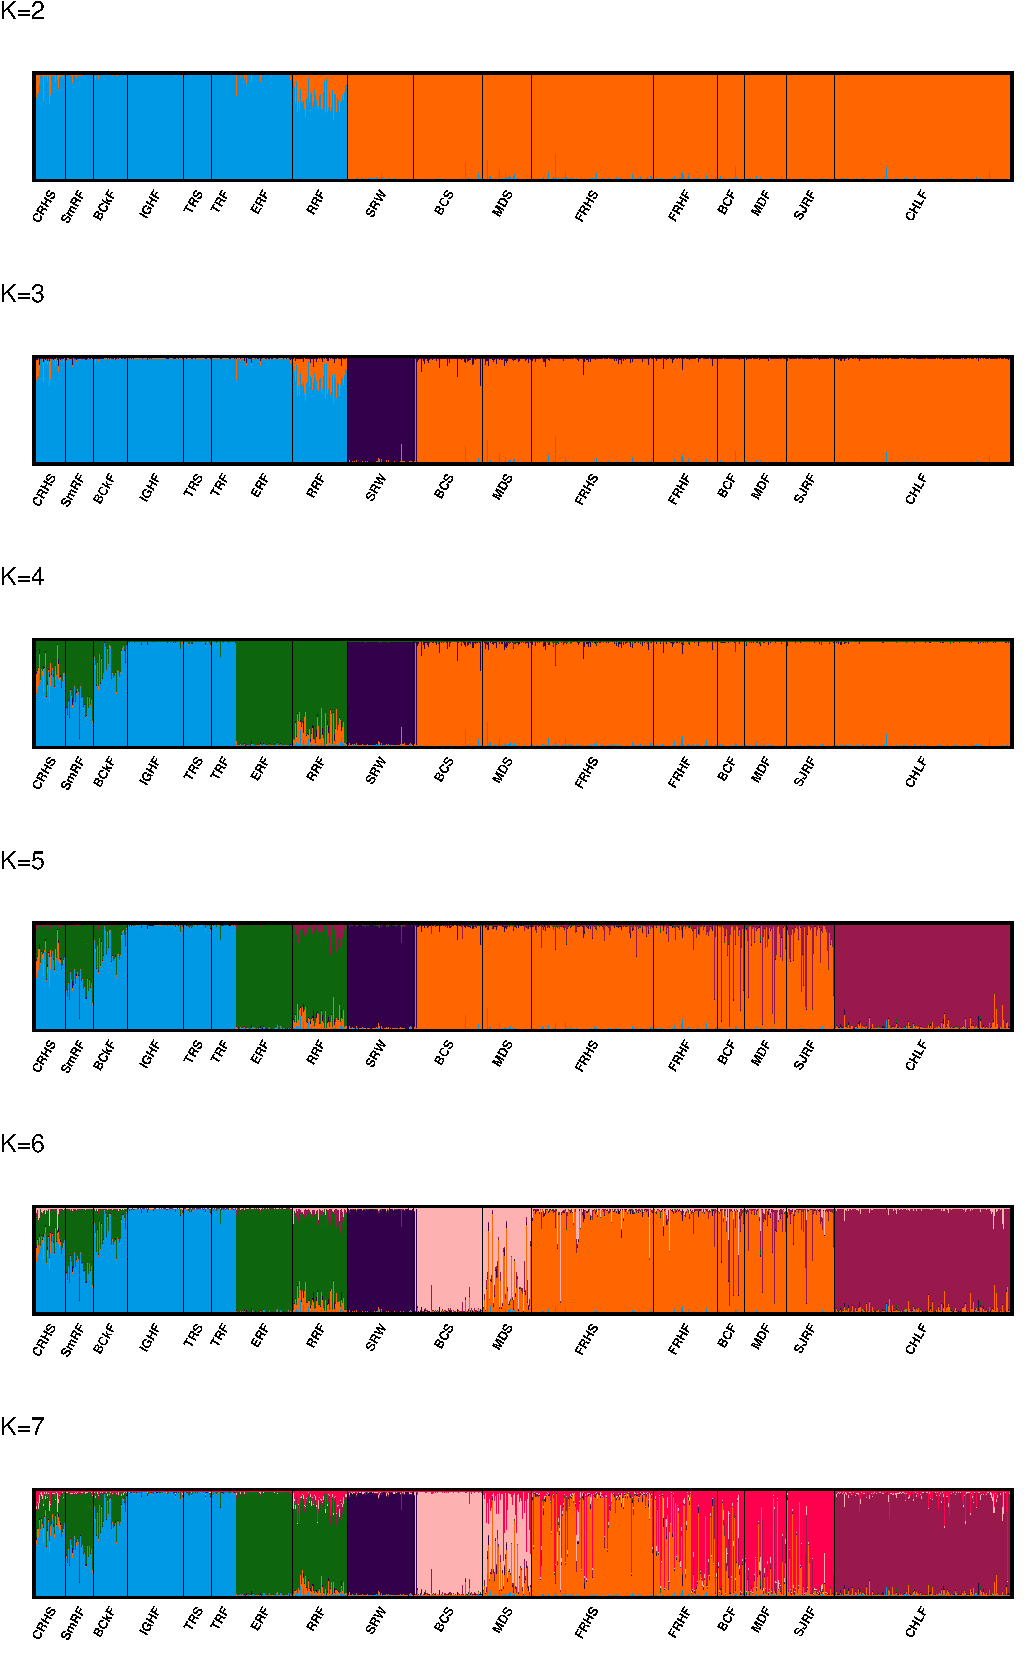
\includegraphics[width=0.48\textwidth]{images/clumpak-crop.pdf}
\end{center}
\caption[\structcap]{\structcap}
\label{fig:struct}
\end{figure}
%%%%%%%%%%%%%%%%%%%%%%%%%
The late-fall run collection (CHLF) appears as a separate cluster at $K$ values
as low as 4, with the inclusion of the LFAR markers.  This is notable, since accurately discriminating between the late-fall and
fall-run Chinook salmon of the Central Valley has been impossible with previously used genetic marker sets.
Another noteworthy feature appears at $K=7$, with STRUCTURE separating the fall-run reporting unit
into two clusters that do not correspond exactly with the individual
collections within the reference baseline. For example, fish from the
cluster that predominates in the FRHS collection are also found in the FRHF and MDS collections.


\subsection*{Power for genetic stock identification and population assignment}

Leave-one-out cross-validation (self-assignment) analysis demonstrates that this
reference baseline provides a high degree of accuracy for distinguishing the major
groups of Chinook salmon in California.  The results of the analysis are summarized
in a self-assignment matrix (Figure~\ref{fig:gsi}b).
This figure shows the collections divided into the seven different reporting groups:
SO-NCal-Coast,  Klamath-Trinity, Cent-Cal-Coast,
CV-Winter, CV-Spring, CV-Fall, and  CV-Late-Fall.  These groupings correspond
largely to the divisions in the data found by STRUCTURE, and they also correspond
with divisions amongst the stocks as defined for management, and, as seen in
Figure~\ref{fig:gsi}b, they correspond with groups of populations that can be reliably distinguished
from one another for population assignment.

Overall, of the 1636 fish in the reference baseline, 1612 (98.5\%) were correctly
assigned to their reporting unit of origin, while 24 (1.5\%) were incorrectly assigned.
Four of those 24 misassignments which involved fish being incorrectly assigned to
SRW, were clearly fish from SRW that had been incorrectly sampled into a different
collection, likely due to straying. (This is evident because SRW are so distinct that it is highly improbable they
would be incorrectly identified).  Of the remaining 20 misassignments,  8 involved fish from the
CHLF (late fall run) collection being misassigned to the CV-Fall reporting unit and 6 were
fish from the MDS (Mill-Deer spring run) collection being assigned to the CV-Fall reporting unit.
It is possible that some of these misassignments represent CV-Fall fish that were incorrectly
sampled as CHLF or MDS; however, unlike with SRW,  we  cannot conclude that
confidently, as there is some degree of overlap in likelihood values between the two.

While fish from CHLF were found to misassign at a rate of 2.7\% (8/300) and MDS at a rate
of 7.1\% (6/84) to CV-Fall, misassignment in the other direction occurs at a much lower
rate---that is, fish from the CV-Fall are misassigned to CHLF at a rate
of only 0.6\% (3/508) and to the CV-Spring reporting unit (to which MDS belongs) at a rate
of only 0.4\% (2/508).
When assignments are only accepted with a scaled likelihood greater than 0.8,
10 incorrect assignments and 10 correct assigments are discarded.  Thus,
at the 0.8 threshold, the total fraction of correct assignments is 99.1\% (Figure~\ref{fig:eighty}).
Notably with the $>$0.8 criterion, the misassignment rates from the abundant CV-Fall
reporting unit to CV-Late-Fall or to CV-Spring both drop below 0.2\% (1/502).  

As seen in previous studies, FRHS, the Feather River Hatchery
spring-run stock, is considerably differentiated from the remaining spring-run
stocks in the Central Valley (MDS and BCS). This is reflected in the low
misassignment rates of FRHS fish to the CV-Spring, and is also evident in the
STRUCTURE results.   We note, however, that the RoSA markers provide
the differential signal necessary to distinguish
Feather River spring-migrating fish from the other CCV stocks with a predominantly fall-run
genomic background. 

FRHS fish are produced by selecting spring-tagged fish that again return in fall, 
when the hatchery ladder reopens. This results in untagged spring run, fish not 
encountered during the spring trapping season, being used as broodstock for the fall-run program.
This is evident when the assignment matrix is enumerated in
terms of RoSA genotypes (Figure~\ref{fig:rosa-gsi}). In this context, it is clear that the ``fall-run'' hatchery
program in the Feather River generates many spring-run fish and RoSA heterozygotes.
Similarly, in other regions, such as the Trinity River, the RoSA markers are the only reliable means to distinguish fall-
and spring-run fish, as they otherwise share genomic background.

In California, only the Sacramento and  Klamath basins have documented spring-run
salmon and their historical occurrence in other basins has been unclear; however
we identified three additional copies of a
recombinant haplotype that carries half of the RoSA SNPs from both the E and L lineages in the Eel and Russian rivers. No other clear recombinants were identified in the study populations, suggesting that it arose in the California Coastal Chinook Salmon lineage, and providing further evidence of past presence of RoSA haplotypes associated with early migration.





\subsection*{Power for relationship inference}

The `CKMRsim' power analyses for this set of markers demonstrates that they have ample variation
for accurate identification of parent-offspring (PO) and full-sibling (FS) pairs in almost all
realistic situations. The predicted false positive rates from unrelated pairs for both the
parent-offspring (PO) and full-sibling (FS) relationships are
exceedingly low for all population groups, even when using stringent false negative thresholds as
low as 0.05 (Figure~\ref{fig:fprs}a).
For example, the false positive rate for FS identification is less than one error in 10 million
comparisons of potential siblings in the California Chinook salmon population with the lowest
heterozygosity (SRW) at a false negative rate of 0.05. 

%%%%%%%%%%%%%%%%%%%%%
\begin{figure*}
\newcommand{\fprcap}{\footnotesize False positive rates (FPRs) as a function of false negative
rates (FNRs) for distinguishing between different relationships. Groupings for panels that are neither a previously defined reporting unit nor a single collection (Table~\protect\ref{tab:samples}) are as follows: TRH = \{TRS, TRF\}; FRH = \{FRHS, FRHF\}; CVF = \{BCF, MDF, SJRF\}.  {\bf (a)} FPRs calculated
using importance sampling of unrelated pairs of individuals being incorrectly categorized as parent-offspring (PO),
full-sibling (FS) or half-sibling (HS) pairs.  {\bf (b)}  FPRs calculated using regular Monte Carlo
sampling of avuncular pairs (AN: aunt-niece, uncle-nephew, etc.) or full-siblings (FS) or half-siblings (HS) being
incorrectly categorized as parent-offspring (PO); as well as FPRs of parent-offspring (PO) pairs or half-sibling (HS)
pairs being incorrectly inferred as full siblings (FS).  In both {\bf a} and {\bf b}, 100,000 Monte Carlo replicates
were simulated.}
\begin{center}
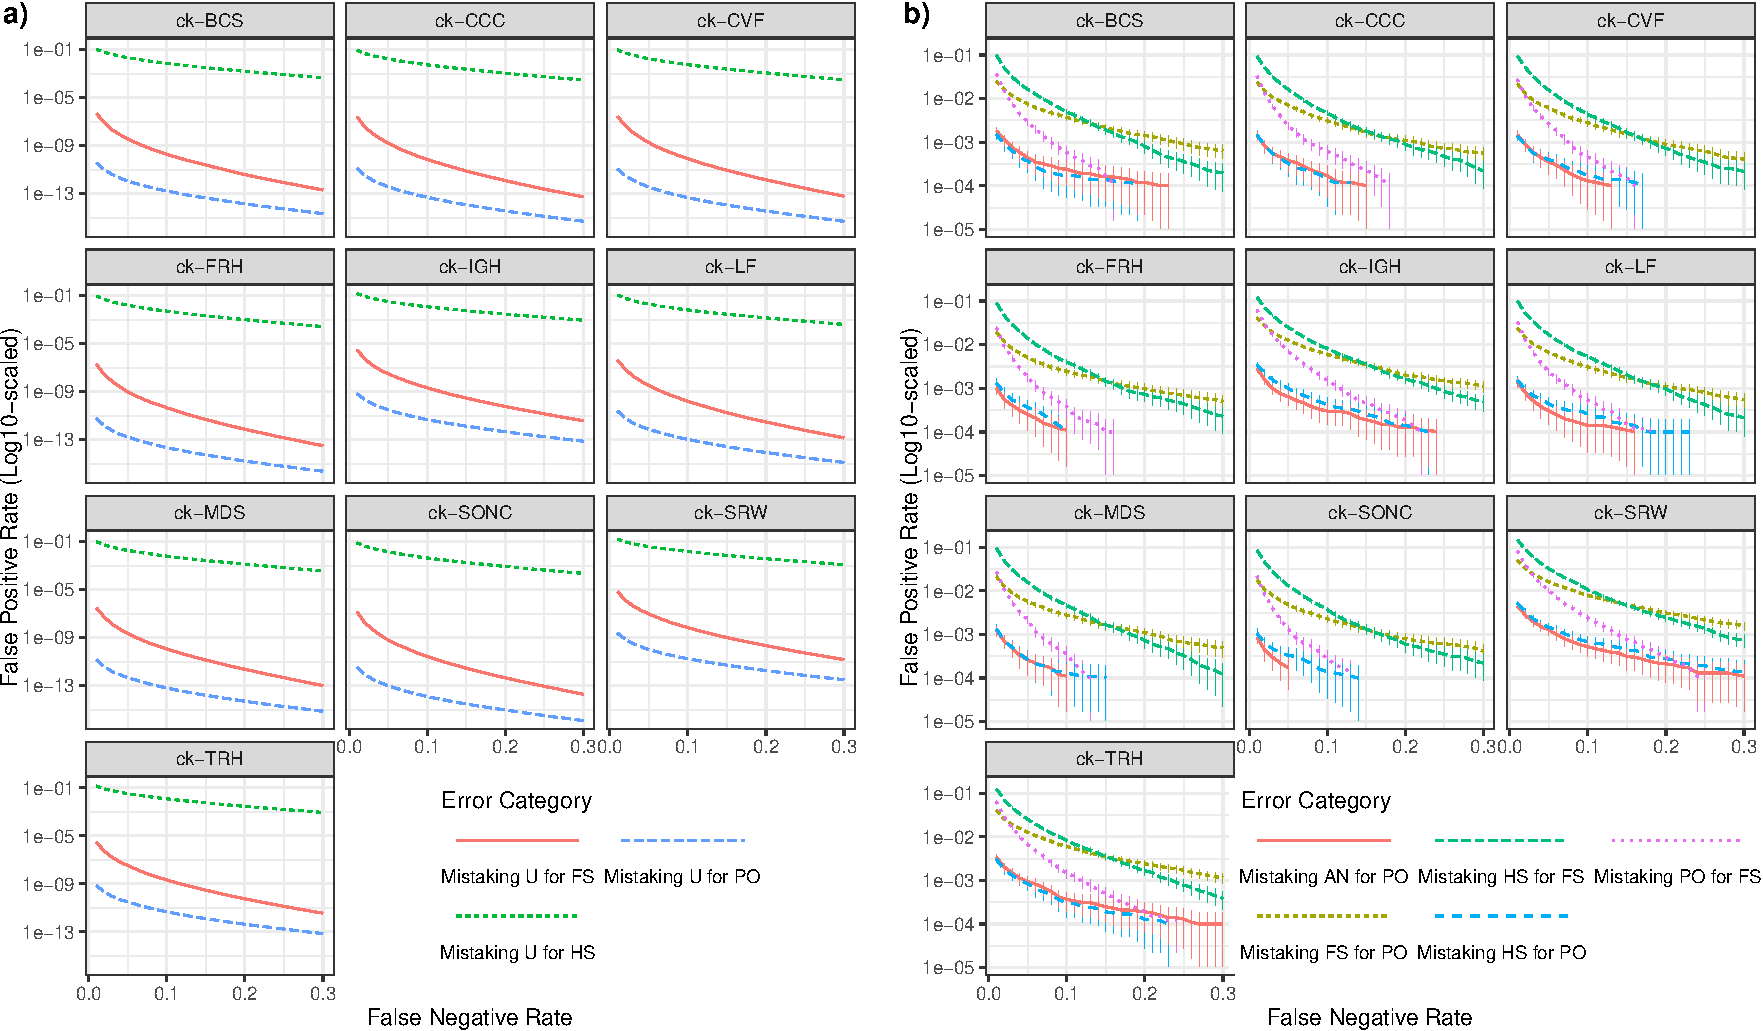
\includegraphics[width=\textwidth]{images/fpr-fnr-figure-crop.pdf}
\end{center}
\caption[\fprcap]{\fprcap}
\label{fig:fprs}
\end{figure*}
%%%%%%%%%%%%%%%%%%%%


Half-sibling (HS) pairs cannot be accurately
distinguished from unrelated pairs in any populations without very large false negative rates
and in very modest-sized studies with very few pairwise comparisons.  

In a reasonably large population, the vast majority of pairs of individuals are expected to
be unrelated, or at least, effectively unrelated, sharing common ancestors only many generations
in the past.  However, a small fraction of pairs will be more recently related, and distinguishing these
kin pairs from target relationships (like PO and FS) must be accounted for.  `CKMRsim' provides
facilities for assessing error rates between different kin groups, and results for these are
summarised in (Figure~\ref{fig:fprs}b). Here, again, focusing on the results for the genetically
depauperate SRW, and using an FNR of 0.1, the chance of incorrectly
categorizing an HS as an FS,  or an FS as a PO is less than 1 in 100. Likewise, 
we can expect PO to be misidentified as FS at a rate of around 1 in 500, and 
HS or Aunts/Uncles to be misidentified as parents at a rate less than 1 in 1000.
Though these rates are much higher than the FPRs for unrelated pairs, they should be
compared to the number of actual non-target kin pairs expected.  For example, in a salmon
population, the number of full aunts or uncles of a fish is unlikely to exceed 50, 
at later life stages,  so a FPR of  $<$0.001 is comfortably low in that case.
Estimation of
error rates between different kin-categories cannot be done in `CKMRsim' using
importance sampling. Consequently, it is difficult to accurately estimate the small
probabilities ($10^{-4}$ or less) in Figure~\ref{fig:fprs}b, as indicated by the error bars,
which represent the estimate $\pm2s$ where s is the estimated standard error of the
mean of the Monte Carlo sample.  However, as noted above, because there are
far fewer related pairs than unrelated pairs, it is not typically essential to
have accurate estimates of very low FPRs for related pairs.  


The presence of multiple alleles at many of these loci improves power for
kin inference compared to a marker panel using only a single SNP at each
amplicon.  To provide a visual display of the difference afforded by using
microhaplotypes compared to single SNPs in this data set, we show the
distribution of log-likelihood ratios for different relationships using our microhaplotype-scored
amplicons, versus using the most heterozygous single SNP from each
amplicon (\ref{fig:ckmr-comp}).  The figures show a considerable increase
in separation between the relationships categories from calling genotypes
as microhaplotypes in these amplicons.

While there is not a currently available method \citep[like that of][]{anderson2006power}) for estimating error rates in
inference of parent-offspring trios with multiallelic marker data, given the substantial amount of statistical power for identifying
PO and FS pairs, which 
require much more statistical power, we hypothesize that PO-trio inference with these markers will be very accurate.








\section*{Discussion}

We describe a novel panel of microhaplotype genetic markers for Chinook salmon
in California that provides sufficient power for highly accurate identification 
of parent and offspring pairs and full siblings, and also allows near-perfect
identification of individuals to population or genetic group of origin in California. 
This set of genetic markers includes multiallelic gene regions with high variability for
relationship inference, gene regions identified in whole-genome sequence data
for increased power for identification of specific populations, and markers that have
long been in use for both GSI and PBT in California \citep{clemento2014evaluation}, by converting them
into so-called 'SNPlicons.' This set of markers lays the foundation for a comprehensive 
genetic monitoring and evaluation effort that facilitates multiple types of inference 
and is flexible and extensible.


This marker set and baseline reference dataset provide
excellent power for identifying fish from all of the Chinook salmon ESUs in California,
as well as individual populations within those ESUs (Figure~\ref{fig:gsi}).
The California Central Valley (CCV) is one of the largest river
basins on the west coast of North America and drains the Sierra Nevada and southern Cascade
mountain ranges. It has the highest diversity of recognized Chinook salmon
ecotypes in the species range, with four named ecotypes, two of which are protected
under the US Endangered Species Act. It is also the source of household water for
tens of millions of California residents and millions of acres of arguably
the most productive and valuable agriculture area in North America. As such, accurate identification of the distinct 
ecotypes of CCV Chinook salmon is of utmost importance for monitoring and
evaluation of individual ecotypes, and for designing and implementing
effective conservation and management actions. This has been challenging,
given the recent common ancestors of these ecotypes \citep{clemento2014evaluation}, and
ongoing migration between subbasins where different ecotypes predominate.

We describe the first set of genetic markers that produces easily replicable data and
that identifies all of the ecotypes in the CCV, including the late-fall-run Chinook salmon ecotype.
The late-fall-run occurs only in the CCV and shares a genomic background with the more
common CCV fall-run salmon ecotype, so has been refractory to previous GSI efforts with other marker types \citep{seeb2007development,clemento2014evaluation,meek2016sequencing,thompson2024genomics}. 


Moreover, we show how the FRH spring-run lineage is
easily identifiable through a combination of traditional GSI and the characterization
of functional genetic markers in the RoSA. Finally, although previous work has described
GSI capabilities that distinguish the natural-spawning CCV spring-run lineages from
each other and their fall-run counterparts with moderately high accuracy, we demonstrate
near complete accuracy in distinguishing these 'stocks'. Moreover, the few fish that are
apparently misidentified (Figure~\ref{fig:gsi}) are likely to be primarily migrants and not true misidentifications.
For example, the three fish that were field-characterized as spring-run from Butte Creek, but are
genetically identified as winter-run salmon clearly carry the winter-run genomic background and
are strays from the winter-run stock, as these could not realistically be misidentified on the 
basis of the genetic data.

Results from the model-based clustering analysis with the program STRUCTURE, revealed patterns 
of population relationships that are coincident with previous work 
\citep{clemento2014evaluation,kinziger2013contemporary}, emphasizing
the distinction between Chinook salmon populations 
in Coastal California and the Central Valley. These analyses also uncover some additional patterns, 
including the clear presence of mixed ancestry in the Coastal California population in the 
Russian River, which is consistent with its location, at the southernmost edge of the 
Coastal Chinook salmon distribution and proximate to the mouth of the Sacramento River 
(the Golden Gate). In the Central Valley, the clustering results emphasize the genetic 
distinction of the SWR population, which is likely at least partially due to 
the extreme bottleneck that it passed through in the 1980s and 1990s \citep{hedrick1994effective}. The inclusion 
of the LFAR markers also resulted in the clear distinction of the CHLF group, which 
is coincident with the long-known phenotypic distinction of this population, but represents a novel 
genetic result. Moreover, at K = 7, the fall-run reporting group breaks into two clusters, 
which are distributed across almost all of the spring and fall-run populations in the 
Central Valley, albeit not equivalently, emphasizing both current and historical migration and 
gene flow between them. 

Examination of the geographic patterns of allele frequencies for the RoSA-associated loci found a
clear instance of the early-migrating haplotype present in the California Coastal Chinook salmon lineage.
This is of note because this lineage does not currently have an early migrating component, although it
has long been speculated that the Eel River, at least, historically harbored early-migrating Chinook salmon,
and early migrating steelhead ({\em O. mykiss}) persist in the basin \citep{bjorkstedt2005analysis}. Moreover, we
discovered several recombinant RoSA haplotypes in both of the CCC populations that indicate a long-standing
presence of both the early- and late-migrating haplotypes in these populations. This is consistent with the
idea that early-migrating populations arise through migration of small numbers of individuals carrying 
E-lineage haplotypes, in either heterozygous or homozygous form, which are subsequently positively selected
when appropriate habitat conditions exist. A similar pattern of recombination, due to long-standing
co-occurence of the E and L haplotypes in heterozygotes, has been previously documented in the Klamath 
River \citep{thompson2020complex}.

%\comment{Maybe discuss: A large fraction of the Feather River
%Hatchery Spring-run (FRHS) collection into a cluster (colored orange in Figure~\ref{fig:struct}).
%A large fraction of the samples from the fall-run hatchery
%program at the Feather River (FRHF) are also members of that same orange cluster, while others
%belong to a cluster composed of other fall-run Chinook salmon. These STRUCTURE results at $K=7$,
%validate the finding that all populations outside of the }

%Although previous work using genome-scale data has shown that many of
%these populations or stocks can be resolved \cite{thompson2020complex,meek2020identifying},
%such data are not practical for most large-scale applications of GSI and PBT, particularly because
%of the much higher costs, longer turnaround time and challenges of producing highly
%replicable datasets with reduced representation and low-coverage whole genome sequencing methods \cite{ali2016rad}.


Previous genetic marker sets for California Chinook salmon had sufficient power for inferring
parent-offspring relationships, but only when both parents were sampled and genotyped.
This marker set considerably increases the capacity for relationship inference in California
salmon, by providing sufficient power for parent-offspring relationship inference, when only
one parent is sampled, and identifying pairs of full siblings when no parents are sampled.
Groups of full siblings larger than two can be identified even more accurately than expressed in Figure~\ref{fig:fprs},
when using statistical approaches that account for the joint relationships between more than two individuals,
such as COLONY \citep{wang2004sibship}.
Although some additional errors might be
expected when related but non-target kin pairs are sampled,  the false positive rates
for these non-target kin pairs are sufficiently small
for almost all realistic scenarios.
Accurate relationship
inference in even the most genetically depauperate Chinook salmon population in California
and rangewide \citep{seeb2007development,clemento2014evaluation} is therefore possible with this marker set.
We note that, as in previous work, it is nearly impossible to identify HS pairs accurately
with data from this, or any standard marker dataset. Accurate identification of HS pairs
typically relies on many hundreds of microhaplotype markers \citep{baetscher2018microhaplotypes} or thousands of SNP markers \citep{hillary2018genetic}. 

As sequencing costs drop, whole genome sequence (WGS) data may become the preferred
data type for salmon genetics. If so, it may become possible to include
all the >200 genetically distinct Chinook salmon populations in North America within a
single standardized reference baseline constructed with WGS data
that performs equally well at broad and regional scales \citep{desaixINPRESSpopulation}.
Such an approach would be highly flexible and extensible, as it would allow for the 
assignment of unknown-origin fish using
just about any marker type, including reduced representation DNA sequencing
\citep[e.g.,~RADseq,][]{meek2020identifying,thompson2024genomics},
as the variation used by such region-specific panels of markers should be contained within the WGS baseline dataset.
For the present, however,
baselines tailored to specific regions are essential for regional management questions and
targeted sequencing approaches have proven to be the most practical for large-scale
applications of either GSI, PBT or an integrated monitoring program \citep{beacham2021parentage}.



\section*{Acknowledgements}
Many people from various agencies and watershed groups contributed to the collection
of the samples analyzed here, including staff from the California Department of Fish and Wildlife,
National Marine Fisheries Service, US Fish and Wildlife Service, US Army Corps of Engineers and 
Pacific States Marine Fisheries Commission. We also thank Elena Correa, Nicole Anderson and Libby
Gilbert-Horvath for contributions to data collection. The manuscript was improved by comments from
Jeff Rodzen and from two anonymous referees. USDA is an equal opportunity provider and employer. Mention of trade names
or commercial products in this publication is solely for the purpose of providing specific
information and does not imply recommendation or endorsements by the U.S. Department of Agriculture.